\documentclass[../../../main.tex]{subfiles}
\begin{document}

As mentioned in the previous section, to print non-planar printing, it is not enough to obtain a G-code. 
Paraphrasing Aristotelian metaphysics: after generating the non-planar G-code, the printer possesses the \textit{potentiality} to print in a non-planar fashion. 
However, for this potentiality to become \textit{actuality}, specific hardware modifications must be implemented.
Specifically, the nozzle. 
This section will show the different extruders used and how they were adapted for operation.

\subsection{Nozzle design}

The 3D printer used in this project was a Creality Ender 3 v1. 
It includes an extruder like the one shown in \cref{fig:nozzle}. 
This extruder is screwed onto a block made of heat-conductive material with an internal resistive heater, along with a thermistor or thermocouple for precise temperature control.

\begin{figure}[!htbp]
    \centering
    \\includegraphics[width =0.7\textwidth]{imgs/nozzle.svg.pdf}
    \caption{Drawing of the dimensioned cross-section of the Creality Ender 3 v1 nozzle.}
    \label{fig:nozzle}
\end{figure}

The figure shows that the extruder is very thick and flattened at the tip. 
The height of the extruder neck is slightly more than 3 \textit{mm}, and the outer walls of the extruder form an angle of $\approx 53^{\circ}$.
Suppose the penetration, $P(d)$, is defined as the distance that an extruder can penetrate parallel to a printed column at a distance \textit{d} without hitting it. In that case, this extruder has a maximum penetration of 8 \textit{mm} at a distance of 3.5 \textit{mm}, where the conical surface ends. 
However, its penetration function would be as follows:
\[
P(d)=
\begin{cases}
\frac{3.38}{R_e}\,d & 0 \le d \le R_e,\\[4pt]
8 & d > R_e
\end{cases}
\quad (\text{mm}).
\]
Where $R_e = 3.5\; mm$ is the radius of the extruder and \textit{d} is the horizontal distance.
Once the radius of the extruder is reached, the penetration is constant and equal to the length of the extruder.
Penetration determines the geometry that can be printed non-planar with an extruder. 
In this case, geometries with a height greater than 4 mm cannot be printed if there are printed structures within a radius of $R_e$. 
It is obvious that this extruder cannot be used to print the structures proposed in this work. 
An extruder with greater penetration is required. 
The greater the penetration slope, the better.

Since conventional 3D printers are designed to print layer by layer, it makes no practical sense to increase the length of the extruder. 
The only geometry that makes sense to modify for planar printing is the diameter of the nozzle. 
When an extruder becomes longer, the distance between the gears that push the filament and the outlet hole increases, which can cause pressure losses in the liquid plastic. 
For this reason, long extruders are not found among the products offered by manufacturers of extruders for 3D printers. 
Therefore, a solution outside of 3D printing had to be found. 
The first solution proposed was to use an airbrush nozzle screwed onto an adapter. 
Normally, these nozzles are very small, typically M2, and the hot block thread is M6. 
An adapter is therefore needed between the two. 
The company NA3D, Czech Republic, sells both parts together: Brass M6 nozzle with airbrush tip. 
The nozzle is made of high-quality brass and stainless steel, which is resistant to rust and corrosion. 
Both parts were bound with high-temperature epoxy putty from JB Weld, United States (HighHeat Stick, Prod. code 8297). 
This putty is designed to withstand temperatures up to 290$^{\circ}$.
In \cref{fig:nozzle2}, a dimensioned drawing of the nozzle is shown.
The diameter of the extruder remains the same, although the company sells different interchangeable sizes. 
The image shows the 0.4 \textit{mm} diameter extruder.

\begin{figure}[!htbp]
    \centering
    \\includegraphics[width =0.7\textwidth]{imgs/nozzle2.svg.pdf}
    \caption{Drawing of the dimensioned NA3D nozzle with airbrush tip.}
    \label{fig:nozzle2}
\end{figure}

It is noticeable that this new extruder is more pointed; therefore, its penetration will be greater. 
If the thread head of the tip is ignored and it is assumed that this area does not affect penetration, its penetration function can be approximated as

\[
P(d)=
\begin{cases}
\frac{6.55}{R_e}\,d & 0 \le d \le R_e,\\[4pt]
9.29 & d > R_e
\end{cases}
\quad (\text{mm}).
\]

Where in this case $R_e = 3.58 \;mm$. 
The penetration slope of this extruder is twice that of a conventional extruder. 
And if it is only considered the tip, it is four times greater.
Since the tip angle is 77$^{\circ}$, this design allows for printing 4 \textit{mm} columns with a separation of slightly more than half a millimetre. 
With the previous extruder, the separation had to be 3.5 \textit{mm}, so this separation has been reduced by 75\%. 
Despite this, the maximum possible penetration is still very small, at 9.29 \textit{mm}. 
This design still limits non-planar printing to structures with very short edges. 
In the structures presented in the previous chapter as an example, it can be seen that many edges far exceed this length. 
Therefore, another, even longer extruder design must be sought. 
The ideal design would be an infinitely long cylinder as narrow as the desired edge thickness.
However, such a design is obviously impossible. 
Therefore, the size of the admissible structures will always depend on the design of the extruder used.

At this point, there are no extruders this long in 3D printing. 
In bioprinting, or low-temperature printing, there are elongated plastic needles; however, they are not suitable for this case as they would melt at the required temperature. 
As a solution to this problem, it is proposed to use hospital syringe refill needles. 
There are designs made entirely of stainless steel, making them suitable for use in high-temperature printing. 
In addition, they are very thin and elongated. 
The problem with these needles is that they are commonly connected to the syringe by pressure, coupling the female conical closure of the needle to the male cylindrical closure of the syringe. 
This configuration does not have any means of preventing slippage or possible fluid leaks.
Therefore, they cannot be used in this way, as the internal pressure of the molten polymer inside the extruder is much higher than the pressures at which these needles normally operate, and they would detach.
However, there are some models that have a Luer-type closure. 
This closure is threaded and is used to avoid the problems of pressure-coupling. 
It ensures that the connection remains fixed, although it does not lock it. 
High pressures can cause the needle to rotate, unscrewing it. 
However, these pressures must be very high and depend on the proper design of the female and male closures. 
Lower pressures can cause the needle to slip slightly and lead to leaks. 
But, as the molten polymer has high viscosity, leaks should not be frequent if the closure is done correctly. 
Although these needles seem to be a promising solution to the problem, they cannot be used without an adapter, as there are no 3D printers with a Luer lock. 
Therefore, an M6 to Luer adapter is required. 
Fortunately, metal adapters with these characteristics are available. 
Both parts were purchased from Ningbo Xinkeda Electronics Co., Ltd., China. 
There are various designs of needles of this type, with different lengths and diameters. 
Several different lengths and diameters were purchased to test which ones work best. 
As these are medical needles, their diameter is specified in Birmingham gauge\footnote{The Birmingham gauge, officially the Birmingham Wire Gauge and often abbreviated as \textit{G} or \textit{ga}, is a unit of wire gauge used to measure the thickness or diameter of wires and tubing, including hypodermic needles and other medical tube products. The reader can find more information about this metric unit and its correlation with millimetres in this \href{https://en.wikipedia.org/wiki/Birmingham_gauge}{page.}}, so needles with the same diameters as conventional extruders are not available, but approximate ones are. 
The adapter used is nickel-plated brass, while the needles are stainless steel. 
\cref{fig:adapter} and \cref{fig:needle} show a detailed view of the adapter and a needle with a Luer lock, respectively. 
It should be noted that certain dimensions may differ slightly from reality due to the accuracy of the 3D model used, but they serve as a supporting visual tool. 
As mentioned above, the dimensions of the needle may vary depending on the model used. \cref{fig:needle} shows an 18-\textit{G} needle.
In addition, \cref{fig:joint} shows a section of the assembly of both parts.


\begin{figure}[!htbp]
    \centering
    \\includegraphics[width =0.8\textwidth]{imgs/adapter.svg.pdf}
    \caption{Dimensioned drawing of the M6-Luer adapter.}
    \label{fig:adapter}
\end{figure}

\begin{figure}[!htbp]
    \centering
    \\includegraphics[width =0.5\textwidth]{imgs/needle.svg.pdf}
    \caption{Dimensioned drawing of a 18-\textit{G} Lure needle.}
    \label{fig:needle}
\end{figure}

\begin{figure}[!htbp]
    \centering
    \begin{subfigure}[b]{0.3\textwidth}
        \centering
        \\includegraphics[width =\textwidth]{imgs/joint_1.svg.pdf}
        \caption{Section of the assembly of the adapter and the needle.}
     \end{subfigure}
     \hspace{1cm}
    \begin{subfigure}[b]{0.25\textwidth}
        \centering
        \includegraphics[width =\textwidth]{imgs/joint.png}
        \caption{3D design of the assembly of the adapter and the needle.}
     \end{subfigure}
     \caption{Assembly of the adapter and the 18-\textit{G} needle}
    \label{fig:joint}
\end{figure}

This proposal was the best found for use as an extruder for high-temperature non-planar printing. 
It can be seen that for this needle, penetration is constant and equal to its length. 
This makes it an ideal candidate for the structures to be printed.

\subsection{Fluid-thermal analysis of the extruder}

Although this design was the best found, it still has its drawbacks. 
As it is a needle used in a field completely different from 3D printing, its design is not optimised for this use case. 
The same argument applies to the adapter. 
As can be seen in \cref{fig:joint}, the end of the adapter does not match the flat internal base of the needle; there is a 2 \textit{mm} gap between the two surfaces. 
This will create a chamber where the fluid will accumulate before entering the needle, which has a cross-section of 1 \textit{mm} in the drawing, while the chamber has a cross-section of 4.11 \textit{mm}. 
In addition, both parts are joined by a wall perpendicular to both, causing the fluid to undergo a very abrupt contraction of the cross-section, increasing the pressure required for the fluid to flow through the needle.


In the extrusion process of molten PLA, the fluid cannot be modelled as a Newtonian fluid. Instead, it behaves as a non-Newtonian, shear-thinning, viscoelastic material whose viscosity strongly depends on the shear rate and the temperature. 
For practical purposes, PLA can be approximated by the \textit{power-law} (Ostwald--de Waele) model:

\begin{equation}
    \tau = K \, \dot{\gamma}^{\,n}, \qquad 0 < n < 1,
\end{equation}

where $\tau$ is the shear stress, $\dot{\gamma}$ the shear rate, $K$ the consistency index, and $n$ the flow index. Both $K$ and $n$ depend on the extrusion temperature.
For laminar, fully developed flow in a capillary tube of radius $R$, length $L$, and volumetric flow rate $Q$, the wall shear rate can be obtained from the Rabinowitsch correction:

\begin{equation}
    \dot{\gamma}_w = \frac{3n+1}{4n} \, \frac{8Q}{\pi R^{3}}.
\end{equation}

The wall shear stress is then given by

\begin{equation}
    \tau_w = K \, \dot{\gamma}_w^{\,n}.
\end{equation}

The resulting pressure drop along the tube is

\begin{equation}
    \Delta p_{\text{tube}} = \frac{2L}{R} \, \tau_w
    = \frac{2L}{R}\,K\left( \frac{3n+1}{4n}\,\frac{8Q}{\pi R^{3}} \right)^{n}.
\end{equation}

This expression can be applied to both the upstream feeding tube ($D_1 = 4 \, \text{mm}$, $R_1 = 2 \, \text{mm}$) and the downstream nozzle ($D_2 = 1 \, \text{mm}$, $R_2 = 0.5 \, \text{mm}$), each with their respective lengths $L_1$ and $L_2$.

In addition to the capillary pressure losses, a significant contribution arises from the contraction from the large tube into the nozzle. 
For polymer melts, this pressure drop is dominated by \textit{extensional flow} rather than inertia, and thus the classical correlation 
\(
\Delta p = K_c \tfrac{1}{2}\rho v^2
\) 
is not appropriate.
The standard rheological procedure to quantify this effect is the \textit{Bagley correction}, which consists of measuring the pressure drop $\Delta p$ for different nozzle lengths $L_2$ and extrapolating to $L_2 \to 0$. The intercept corresponds to the contraction pressure drop, $\Delta p_{\text{entry}}$.

In the absence of experimental data, the entry loss can be approximated in the form

\begin{equation}
    \Delta p_{\text{entry}} \approx C(n,\beta)\,K\,\dot{\gamma}_{\text{char}}^{\,n},
\end{equation}

where $\beta = D_2/D_1$ is the contraction ratio, and the characteristic shear rate can be estimated as

\begin{equation}
    \dot{\gamma}_{\text{char}} \sim \frac{8Q}{\pi R_2^3}.
\end{equation}

The coefficient $C(n,\beta)$ depends strongly on the contraction geometry (sharp edge versus rounded entry) and must typically be determined experimentally or by numerical simulation.
Therefore, the total extrusion pressure required by the extruder is the sum of all contributions:

\begin{equation}
    \Delta p_{\text{total}} =
    \underbrace{\Delta p_{\text{tube1}}}_{\text{feeding tube}}
    + \underbrace{\Delta p_{\text{entry}}}_{\text{contraction}}
    + \underbrace{\Delta p_{\text{tube2}}}_{\text{nozzle}}.
\end{equation}

The contraction geometry plays a critical role: rounded entrances can substantially reduce the contraction pressure drop compared to sharp-edged nozzles.
For this reason, conventional extruders are designed with a smooth section reduction, see \cref{fig:nozzle}. 
Chamfers can reduce pressure loss significantly.

Considering molten PLA approximated by a power-law fluid with parameters representative of 210$^\circ$C \cite{polym14132721}:
\[
K = 381.2\ \mathrm{Pa\,s}^{n}, 
\qquad n = 0.91.
\]
Geometry and operating conditions:
\[
\begin{aligned}
&D_1 = 4\,\mathrm{mm}\quad (R_1 = 2.0\times 10^{-3}\ \mathrm{m}), \\
&D_2 = 1\,\mathrm{mm}\quad (R_2 = 0.5\times 10^{-3}\ \mathrm{m}),\\
&Q = 1.0\times 10^{-7}\ \mathrm{m^3\,s^{-1}}\ (=100\ \mathrm{mm^3\,s^{-1}}).
\end{aligned}
\]
For the entry loss at the sharp-edged contraction, the surrogate form can be used
\[
\Delta p_{\text{entry}} \approx C(n,\beta)\,K\,\dot\gamma_{\text{char}}^{\,n},
\qquad \beta = \frac{D_2}{D_1} = 0.25,
\]
with a conservative choice \(C(n,\beta)\approx 2\) (\cite{C_param}) and
\(
\dot\gamma_{\text{char}} \sim \dfrac{8Q}{\pi R_2^{3}}.
\)

With \(\dot\gamma_{\text{char}} \sim \dfrac{8Q}{\pi R_2^{3}} \approx 4.07\times 10^{2}\ \mathrm{s^{-1}}\),
\[
\Delta p_{\text{entry}}
\approx C\,K\,\dot\gamma_{\text{char}}^{\,n}
= 2\,(381.2)\,(4.07\times 10^{2})^{0.91}
\approx 1.81\times 10^{5}\ \mathrm{Pa}.
\]

This value is illustrative and strongly dependent on temperature (via \(K,n\)), flow rate \(Q\), and the entrance geometry (embedded in \(C\)). 
Rounded entries can substantially reduce \(\Delta p_{\text{entry}}\).
Calculating the internal pressure of the polymer inside the extruder during extrusion is a very complex problem, and no studies have focused purely on this issue due to its complexity. 
However, Timothy J. Coogan \cite{pressure} managed to design an extruder to which he attached a pressure transducer and was able to measure pressures between 0.5 and 2 MPa. 
Using these results as a reference, it can be concluded that the increase in pressure required for the polymer to flow through the needle is significant, without considering the pressure required for it to pass through the entire needle.
Therefore, the force that the gears will have to exert to push the filament will be greater due to this increase in pressure. 
To increase the force on the filament, the filament push system was changed. The Creality Ender 3 3D priner includes a Bowden-type push system, which has gears that are very far from the extruder that push the filament. 
Due to the large distance between the point of application of the force and the extruder, the force that can be exerted is lower. 
High clamping values can cause the filament to bend along its path. 
The system was changed to a direct extrusion system, which places these gears next to the hot-end entry, allowing greater force to be exerted on the filament.

In addition to the problem described above, this design has another even more significant issue. 
As mentioned earlier, the extruders in 3D printers are connected to a resistive block that heats up, thereby heating the extruder. 
The difference, and the root of the problem, is that a conventional extruder is 8 \textit{mm} long, while this extruder has a total length of 33 \textit{mm}, 17.8 \textit{mm} of which corresponds to the needle, which is a tube with a wall thickness of 0.1 \textit{mm}. 
This geometry leads to such a large temperature gradient from the hot block to the tip of the needle that the polymer solidifies inside the needle, clogging it.

A thermal simulation was performed to study the temperature distribution in the needle when it is heated at the maximum temperature allowed by the printer, 500 \textit{K}. 
The adapter was considered an ideal element, with no heat loss on any of its sides, to simplify the simulation. The polymer inside the needle was also not considered. The boundary conditions used were:

\begin{itemize}
    \item Upper face at a constant temperature of 500 \textit{K}.
    \item Heat flow on the faces in contact with the air with a convection coefficient of 10 \textit{W/m²/K}, corresponding to calm air, and a standard ambient temperature of 300 \textit{K}.
    \item Initial extruder temperature at 300 \textit{K}.
\end{itemize}

The material used was a generic steel with the following properties:

\begin{itemize}
    \item Density = 7900 \textit{kg/m³.}
    \item Thermal conductivity = 50 \textit{W/m/K}.
    \item Specific heat = 500 \textit{J/kg/K}.
    \item Expansion coefficient = 12 $\mu m/m/K$.
\end{itemize}

The results obtained are shown in \cref{fig:temp}

\begin{figure}[!htbp]
    \centering
    \includegraphics[width =0.4\textwidth]{imgs/temp.png}
    \caption{Temperature distribution in the needle heated to 500 K on its upper surface.}
    \label{fig:temp}
\end{figure}

The image shows that the tip of the needle is at a temperature of 438 \textit{K} (165$^{\circ}$), which is lower than the melting point of PLA (453 \textit{K} / 180$^{\circ}$). 
Half of the needle is at a temperature below that limit, so it would be solidified. 
In reality, the temperature distribution would be much lower, as heat losses in the adapter and the polymer inside have not been taken into account. 
If the polymer were taken into account, part of the heat intended to heat the needle would also be used to heat the polymer, further lowering the temperature. 
Furthermore, if the polymer were in motion, it could be considered as forced cooling of the tube. 
Therefore, the needle temperature would have to be reduced even further. 
However, even in the ideal case studied, it is clear that this extruder design cannot be used.

The first solution proposed was to use a polymer with a lower melting point. 
Polycaprolactone (Facilan™ PCL 100 Filament, The Netherlands) was used, a biodegradable aliphatic polyester with a melting temperature of 60$^{\circ}$ and widely used in bioprinting to manufacture scaffolds. 
It was possible to extrude material through the needle, but due to its low viscosity, it is not feasible to use this material for printing in the air without support.
Therefore, the following solution was proposed to solve the thermal problem: to heat the needle externally.

\subsection{Needle heating system}

Due to the design constraints of the extruder, heating the nozzle externally is a very challenging task. 
At the time of writing this manuscript, there is no commercial solution nor any scientific study for actively heating nozzles. 
The closest proposal to the one sought is the heating system used in industrial plastic extrusion machines. 
These machines use thermal blankets or induction coils to maintain a uniform temperature throughout the entire extrusion system. 
This solution does not apply to this case because these machines have no space restrictions, the tubes in these machines are several orders of magnitude larger than the needle used, and many different configurations are allowed.
The main design constraint of the heating system to be designed is that it must be as thin as possible. 
The wider the heater, the less penetration the needle will have. 
It would not make sense to use such a long, thin needle and add a thick resistive element, as this would diminish the entire purpose of the needle. 
Another constraint to consider is that the system must be very small, just like the needle. 
The ideal solution would be a ceramic thermal blanket that would wrap around the entire needle and have an infinitesimal thickness. 
Unfortunately, nothing like this exists.
Furthermore, it should be noted that the smaller the volume of the heater, the lower its thermal capacity ($C = Q/\Delta T = \rho c_p V$) will be and, therefore, the greater the heat loss it will suffer due to contact with cold air, reducing the heat it can transmit to the needle. 
Therefore, it will be necessary to use an element that is large enough for the conductive heaters to be effective, but as small as possible so as not to alter the thickness of the needle + heater assembly.
The proposed solution was to use Nichrome wire to make a coil around the needle and pass an electric current through the coil. 
Thanks to the Joule-Lenz law, the coil heats up, in turn heating the needle.

Nichrome is an alloy of 80\% nickel and 20\% chromium with a melting point of around 1400$^{\circ}$. 
Its high electrical resistivity ($\rho = $ 100 $\times10^{-8}\Omega \cdot m$, almost 60 times greater than copper) and very low temperature coefficient of resistance ($\alpha = $ 0.0004/$^{\circ}C$) make it an ideal candidate for use as a heating element\cite{nicrom}. 
In fact, Nichrome is the oldest documented form of resistance heating alloy. Furthermore, because of its high ductility, Nichrome wires can be made with very low thicknesses. Since it is a material that is stable at very high temperatures and can be obtained with a very small cross-section, it is the most suitable choice for use in this case study. 
The smaller the wire cross-section, the greater its electrical resistance and, therefore, the lower the current required to reach the desired temperature. 
However, as mentioned above, the smaller the cross-section, the more energy must be supplied to the wire to heat the tube to the target temperature. 
This is because the smaller the amount of material, the lower the thermal capacity. 
In addition, it should be noted that, as it is a wire, it will have a greater surface area in contact with the cold air than with the tube. 
This further reduces heat transfer. However, because nichrome is stable at very high temperatures and its resistance remains practically constant with temperature, it is not a problem to heat it to a high temperature, as long as it is below the melting point. 
Therefore, it is preferable to use a small section so as not to increase the section of the needle and wire combination too much and raise the temperature of the wire too high. 
For this project, 0.2 \textit{mm} section nichrome wire (Microlog, Spain) was used.

The cross-sectional area of the thread is not the only parameter that affects its strength; its length also plays a role. The longer the thread, the greater its strength. 
For a thread with section $d_{wire} = 0.2\;mm \rightarrow r = 0.1\;mm = 1\times10^{-4}\; m$, the resistance as a function of wire length can be written as
\begin{equation}
R_{\mathrm{NiCr}}=\rho \cdot \frac{L_{\mathrm{w}}}{A_{\mathrm{NiCr}}}=\rho \cdot \frac{L_{\mathrm{w}}}{\pi r^2}=100 \times 10^{-8} \cdot \frac{L_{\text {w }}}{\pi\left(10^{-4}\right)^2}=31.8 \cdot L_{\text {w }} \Omega.
\end{equation}

Once the resistance of the wire and the desired temperature are known, an approximate calculation of the required length can be made based on the electrical current.  
Knowing that the tube loses heat to the air through convection and radiation, the power required to heat the tube in a steady state can be expressed as:
\begin{equation}
P_{\text {req }}=\underbrace{h A_{tube}\left(T-T_{\infty}\right)}_{\text {convection }}+\underbrace{\varepsilon \sigma A_{tube}\left(T^4-T_{\infty}^4\right)}_{\text {radiation }}.
\end{equation}

The expression for electrical power is $P = I^{2}R$.
If both powers are equalised, $P_{req} = P$, the following expression is obtained:

\begin{equation}
I\left(L_w\right)=\sqrt{\frac{P_{\text {req }}}{R_{NiCr}}} = \sqrt{\frac{h A_{tube}\left(T-T_{\infty}\right)+\varepsilon \sigma A_{tube}\left(T^4-T_{\infty}^4\right)}{31.8 \cdot L_w}}
\end{equation}

If it is considered that the target temperature is $T = 200^{\circ}$, the ambient temperature is $T_\infty = 25^{\circ}$, natural air convection ($h = 10\;W\cdot m^{-2}\cdot K^{-1}$) and an emissivity of the surface corresponding to an oxidised metal ($\varepsilon = 0.7$). 
It is possible to calculate how electrical parameters vary depending on the wire's length, see \cref{fig:I_lw}

\begin{figure}[!htbp]
\centering
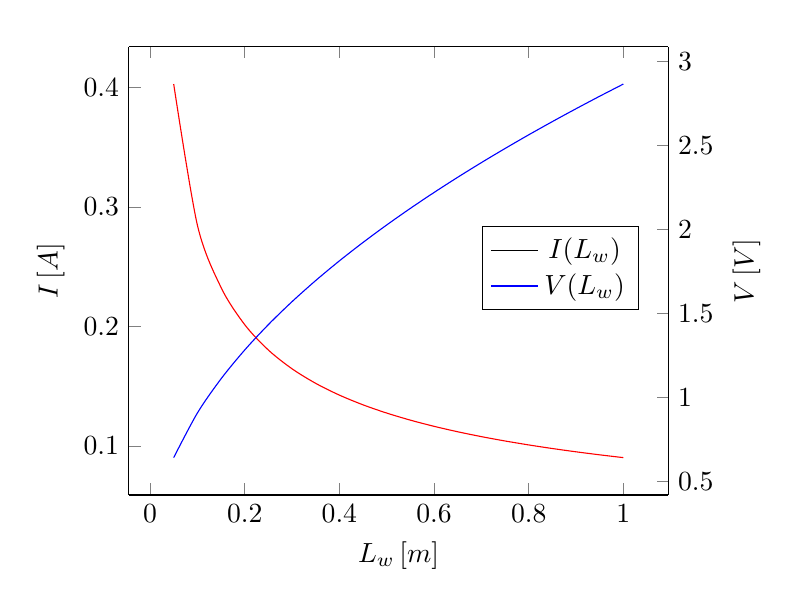
\begin{tikzpicture}
\begin{axis}[
  axis y line*=left,
  axis x line*=bottom,
  xlabel={$L_w\,[m]$},
  ylabel={$I\,[A]$},
]
\addplot[smooth,red]
  coordinates{
 (0.05,0.4029283633566794)
 (0.1,0.28491337806190525)
 (0.15,0.23263079904811423)
 (0.2,0.2014641816783397)
 (0.25,0.18019504210565412)
 (0.3,0.16449481551976664)
 (0.35,0.15229260651657778)
 (0.4,0.14245668903095263)
 (0.45,0.1343094544522265)
 (0.5,0.1274171362091035)
 (0.55,0.12148747260419011)
 (0.6,0.11631539952405712)
 (0.65,0.11175222110933025)
 (0.7,0.10768713479244675)
 (0.75,0.10403565606633536)
 (0.8,0.10073209083916985)
 (0.85,0.09772448245157894)
 (0.9,0.09497112602063508)
 (0.95,0.09243810617673699)
 (1.0,0.09009752105282706)
  }; \label{plot_one}
\end{axis}

\begin{axis}[
  axis y line*=right,
  ylabel={$V\,[V]$},
  ylabel near ticks,
  axis x line*=top,
  xticklabels={},
legend style={at={(0.8,0.6)},anchor=north}
]
\addlegendimage{/pgfplots/refstyle=plot_one}
\addlegendentry{$I(L_w)$}
\addplot[smooth,blue]
  coordinates{
    (0.05,0.6406560977371204)
    (0.1,0.9060245422368587)
    (0.15,1.109648911459505)
    (0.2,1.2813121954742408)
    (0.25,1.4325505847399502)
    (0.3,1.5692805400585736)
    (0.35,1.6950167105295106)
    (0.4,1.8120490844737174)
    (0.45,1.9219682932113613)
    (0.5,2.0259324657247455)
    (0.55,2.124815895847285)
    (0.6,2.21929782291901)
    (0.65,2.3099184103298565)
    (0.7,2.3971156204798647)
    (0.75,2.4812503971820985)
    (0.8,2.5626243909484816)
    (0.85,2.641492760666179)
    (0.9,2.718073626710576)
    (0.95,2.7925551875992243)
    (1.0,2.8651011694799005)
  };
\addlegendentry{$V(L_w)$}
\end{axis}
\end{tikzpicture}
\caption{Variation in the intensity and voltage required to achieve the required power depending on the length of the wire}
\label{fig:I_lw}
\end{figure}

The maximum length of wire that can be used is equivalent to the length of the wire when winding without space between the turns. 
The maximum number of turns will be equal to 
\[
N_{max} = \frac{L}{d_{wire}}.
\] 
Therefore, the maximum length of the wire will be equal to 
\[
[L_{wire}]_{Max} = 2\pi(R_{ext}+d_{wire}/2)N_{max}.
\] 
In the case of the needle in \cref{fig:needle}, the maximum number of turns will be 89 and the maximum length of the wire will be 391 \textit{mm} ($\sim$0.4 \textit{m}).
Therefore, the maximum current needed would be 0.14 \textit{A}, ideally.
These values are illustrative and only serve to give an idea of the order of magnitude of the current needed to reach this state. 
But in reality, the length of the cable from the terminals to the coil would have to be added to the length of the coil, so the actual length would be greater and the current required would also be greater. 
However, a certain length would have to be deducted, as it would not be possible to achieve a perfect winding. 
These calculations have been made for an ideal stationary case in which there are no heat transmission losses between the nichrome and the needle. 
However, in reality, as mentioned above, this heat transmission is very low, meaning that the temperature to which the nichrome must be heated is higher.
Calculating the temperature to which the wire should be heated is actually a very complicated problem that depends on too many factors, especially environmental ones, making it useless to solve.

Although the above calculations are not reliable, they provide an initial idea of the electrical values required. 
In view of the fact that the amperage will always be less than 0.5 \textit{A}, it was proposed to make a PID controller with Arduino to control the temperature at which the needle is heated and keep it the same as the printer temperature. 
Arduino boards are capable of generating output currents of up to 500 \textit{mA} and 5\textit{V}, values that should be sufficient for this case. 
The idea is to use a feedback-based control loop mechanism to vary the output current supplied to the wire by modulating the pulse angle (PWM) until the desired temperature is reached in the tube. 
To achieve this, it is necessary to monitor the actual temperature of the tube and use that value in the PID function to calculate the PWM that should be applied at any given moment.

Measuring the temperature of something so small is very complicated. 
One must bear in mind that the aim is to calculate the temperature of a tube approximately 1 \textit{mm} thick, wrapped in a very hot wire. 
Thermographic cameras available on the market are not capable of measuring such small surfaces unless the distance to the object is very short. 
Also, there may be many degrees of temperature difference between the nichrome wire and the tube, so the high temperature of the nichrome would add a lot of noise to the camera's measurements. 
Furthermore, communication between the software needed to read the cameras and Arduino can be very complicated, and even unfeasible. 
Therefore, the use of thermal imaging cameras for this task was ruled out. 
The remaining option is to use contact temperature measurement elements. 
The problem that arises in this case is that there are no thermocouples small enough. 
If the temperature is to be measured during printing, it cannot be done inside the tube, so the thermocouple would have to be attached to the outer surface of the needle, which would therefore have to have a flat surface. 
As the needle is a tube, the contact surface between the needle and the thermocouple is further reduced, making it more difficult to read. 
Furthermore, adding an additional element to the needle would increase its width, which is something that needs to be avoided to maintain penetration. 
Therefore, it does not seem feasible to measure the temperature during printing either. 
At this point, two alternatives were proposed. 
The first was to measure the temperature of the adapter and relate it to the temperature of the tube. 
As it is bigger, the contact surface between the adapter and the sensor is higher, and therefore the measurements would be more accurate. 
Furthermore, it would not interfere with printing as the sensor would be located outside the printing area. 
The problem with this proposal is that the adapter, being in contact with the printer's hot block, would be at the same temperature as the latter. 
Therefore, the temperature measurements would always be the same as those of the printer. 
It would therefore be better to place the sensor at the base of the needle. 
Besides, as it is flat, the contact surface would be almost total. 
The second alternative was to relate the electrical values to the temperature of the tube experimentally and, once this relationship had been established, to control the temperature of the tube by controlling these values. 
To do this, a sensor would have to be placed at the tip of the needle, the current varied and the heating of the needle monitored. 
This proposal is much simpler, as it would eliminate the need to constantly monitor the temperature of the needle. As it was the simplest, it was the one chosen.
To measure the temperature, the smallest flat thermistor and point thermocouple available on the market were purchased. 
Specifically, the thermistor chosen was a PT100 platinum thin-film RTD thermistor with a contact surface area of 2x2.3 \textit{mm}, capable of reading temperatures between -50 and 300$^{\circ}C$ (Product number NB-PTCO-160, TE Connectivity Measurement Specialties, United States).
In addition, a type K thermocouple with a 0.5 \textit{mm} diameter AISI321 stainless steel sheath capable of reading temperatures up to 250$^{\circ}C$ (Product number 406-480, TC Medida y Control de Temperatura, S.A., Spain) was also purchased.

\subsection{Heating system assembly}

Once it has been decided how the needle will be heated, it must be assembled.
As the tube and wire are metallic, Kapton tape was used as electrical insulation between the two metals to prevent short circuits.
Kapton was chosen because it is a paraffin that is stable up to 400$^{\circ}C$. 
Once the tape has been attached to the extruder, the needle is wound. The winding is done manually, ensuring maximum tension on the wire at all times, and is carried out until the entire length of the needle is covered, leaving 3 \textit{mm} free at the tip to place the thermistor. 
Once the winding was complete, it tended to return to its natural shape. 
In order to apply permanent deformation to the winding, the free end is tensioned so that it compresses the winding for 10 minutes. 
After that time, the material did not tend to stretch.
Behind the assembly, both ends of the thread were connected to a 0-30\textit{V}/0-5\textit{A} variable power supply to check whether the heating system actually works. 
Due to human error, the power supply was preset to higher current values than necessary, raising the temperature of the nichrome so much that the Kapton melted, but no short circuit occurred. 
Thanks to this error, it was discovered that Nichrome generates a layer of chromium oxide ($Cr_2O_3$) when heated, which acts as a dielectric coating and therefore makes it unnecessary to use Kapton between the winding and the tube.
Although the oxide layer electrically insulates the nichrome, it could break down with thermal cycles, leaving the Nichrome exposed. 
This is not really a problem in terms of contact between the steel and the nichrome because Nichrome is a better conductor of electricity than steel. 
Therefore, the current will always tend to flow through the nichrome.

Once the winding is complete, the lower end of the winding lies on the bed, see \cref{fig:heating} \textcolor{blue}{A}. To prevent this part from colliding with the already printed elements, it is folded over the winding so that the lower free end is at the same height as the upper free end,  see \cref{fig:heating} \textcolor{blue}{B}. 

\begin{figure}[!htbp]
    \centering
    

% Gradient Info
  
\tikzset {_gfzs0ycvr/.code = {\pgfsetadditionalshadetransform{ \pgftransformshift{\pgfpoint{0 bp } { 0 bp }  }  \pgftransformrotate{0 }  \pgftransformscale{2 }  }}}
\pgfdeclarehorizontalshading{_avad09siq}{150bp}{rgb(0bp)=(0.96,0.96,0.96);
rgb(37.5bp)=(0.96,0.96,0.96);
rgb(42.75bp)=(0.86,0.86,0.89);
rgb(49.75bp)=(0.72,0.73,0.78);
rgb(57.5bp)=(0.87,0.87,0.89);
rgb(62.5bp)=(0.96,0.96,0.96);
rgb(100bp)=(0.96,0.96,0.96)}

% Gradient Info
  
\tikzset {_azejiuc9f/.code = {\pgfsetadditionalshadetransform{ \pgftransformshift{\pgfpoint{0 bp } { 0 bp }  }  \pgftransformrotate{-270 }  \pgftransformscale{2 }  }}}
\pgfdeclarehorizontalshading{_93j7eyhmf}{150bp}{rgb(0bp)=(1,1,1);
rgb(37.5bp)=(1,1,1);
rgb(62.5bp)=(0,0,0);
rgb(100bp)=(0,0,0)}
\tikzset{_e2p0z38cf/.code = {\pgfsetadditionalshadetransform{\pgftransformshift{\pgfpoint{0 bp } { 0 bp }  }  \pgftransformrotate{-270 }  \pgftransformscale{2 } }}}
\pgfdeclarehorizontalshading{_p9zktzwrj} {150bp} {color(0bp)=(transparent!0);
color(37.5bp)=(transparent!0);
color(62.5bp)=(transparent!10);
color(100bp)=(transparent!10) } 
\pgfdeclarefading{_kzlxmvcsz}{\tikz \fill[shading=_p9zktzwrj,_e2p0z38cf] (0,0) rectangle (50bp,50bp); } 

% Gradient Info
  
\tikzset {_xnc337xop/.code = {\pgfsetadditionalshadetransform{ \pgftransformshift{\pgfpoint{0 bp } { 0 bp }  }  \pgftransformrotate{0 }  \pgftransformscale{2 }  }}}
\pgfdeclarehorizontalshading{_uigf1kp53}{150bp}{rgb(0bp)=(0.96,0.96,0.96);
rgb(37.5bp)=(0.96,0.96,0.96);
rgb(42.75bp)=(0.86,0.86,0.89);
rgb(49.75bp)=(0.72,0.73,0.78);
rgb(57.5bp)=(0.87,0.87,0.89);
rgb(62.5bp)=(0.96,0.96,0.96);
rgb(100bp)=(0.96,0.96,0.96)}

% Gradient Info
  
\tikzset {_4kfiyhkcd/.code = {\pgfsetadditionalshadetransform{ \pgftransformshift{\pgfpoint{0 bp } { 0 bp }  }  \pgftransformrotate{-270 }  \pgftransformscale{2 }  }}}
\pgfdeclarehorizontalshading{_a8foevud7}{150bp}{rgb(0bp)=(1,1,1);
rgb(37.5bp)=(1,1,1);
rgb(62.5bp)=(0,0,0);
rgb(100bp)=(0,0,0)}
\tikzset{_jlmmjjwny/.code = {\pgfsetadditionalshadetransform{\pgftransformshift{\pgfpoint{0 bp } { 0 bp }  }  \pgftransformrotate{-270 }  \pgftransformscale{2 } }}}
\pgfdeclarehorizontalshading{_75h7gvnj1} {150bp} {color(0bp)=(transparent!0);
color(37.5bp)=(transparent!0);
color(62.5bp)=(transparent!10);
color(100bp)=(transparent!10) } 
\pgfdeclarefading{_gsfl3wp05}{\tikz \fill[shading=_75h7gvnj1,_jlmmjjwny] (0,0) rectangle (50bp,50bp); } 
\tikzset{every picture/.style={line width=0.75pt}} %set default line width to 0.75pt        

\begin{tikzpicture}[x=0.75pt,y=0.75pt,yscale=-1,xscale=1]
%uncomment if require: \path (0,300); %set diagram left start at 0, and has height of 300

%Straight Lines [id:da4111860901498777] 
\draw    (439.17,69.25) -- (488.17,57.25) ;
%Shape: Path Data [id:dp3506561022646192] 
\path  [shading=_avad09siq,_gfzs0ycvr] (319.45,53.55) -- (318.66,229.24) .. controls (318.65,229.6) and (318.28,229.9) .. (317.82,229.9) -- (302.87,229.85) .. controls (302.41,229.85) and (302.04,229.55) .. (302.04,229.19) -- (302.84,53.5) .. controls (302.84,53.13) and (303.21,52.84) .. (303.67,52.84) -- (318.63,52.88) .. controls (319.08,52.89) and (319.46,53.18) .. (319.45,53.55) -- cycle (338.07,52.81) -- (286.06,52.66) -- (286.24,11.25) -- (338.26,11.4) -- (338.07,52.81) -- cycle ; % for fading 
 \draw  [dash pattern={on 4.5pt off 4.5pt}] (319.45,53.55) -- (318.66,229.24) .. controls (318.65,229.6) and (318.28,229.9) .. (317.82,229.9) -- (302.87,229.85) .. controls (302.41,229.85) and (302.04,229.55) .. (302.04,229.19) -- (302.84,53.5) .. controls (302.84,53.13) and (303.21,52.84) .. (303.67,52.84) -- (318.63,52.88) .. controls (319.08,52.89) and (319.46,53.18) .. (319.45,53.55) -- cycle (338.07,52.81) -- (286.06,52.66) -- (286.24,11.25) -- (338.26,11.4) -- (338.07,52.81) -- cycle ; % for border 

%Shape: Spring [id:dp5411140102246771] 
\draw   (309.75,56.03) .. controls (316.27,57.64) and (322.77,61.36) .. (322.74,68.24) .. controls (322.68,82) and (296.59,80.87) .. (296.6,77.69) .. controls (296.62,74.52) and (322.71,75.65) .. (322.64,89.41) .. controls (322.58,103.17) and (296.49,102.03) .. (296.51,98.86) .. controls (296.52,95.68) and (322.61,96.82) .. (322.55,110.58) .. controls (322.49,124.34) and (296.4,123.2) .. (296.41,120.03) .. controls (296.43,116.85) and (322.51,117.99) .. (322.45,131.74) .. controls (322.39,145.5) and (296.3,144.37) .. (296.32,141.19) .. controls (296.33,138.02) and (322.42,139.15) .. (322.36,152.91) .. controls (322.29,166.67) and (296.21,165.54) .. (296.22,162.36) .. controls (296.23,159.19) and (322.32,160.32) .. (322.26,174.08) .. controls (322.2,187.84) and (296.11,186.7) .. (296.12,183.53) .. controls (296.14,180.35) and (322.23,181.49) .. (322.16,195.25) .. controls (322.1,209) and (296.01,207.87) .. (296.03,204.69) .. controls (296.04,201.52) and (322.13,202.65) .. (322.07,216.41) .. controls (322.03,224.23) and (313.61,227.24) .. (306.33,227.8) ;
%Straight Lines [id:da28033570455918533] 
\draw    (310.64,56.04) -- (264.29,55.9) ;
%Straight Lines [id:da3319008220898223] 
\draw    (309.52,227.75) -- (263.5,227.36) ;
%Straight Lines [id:da6338243781414553] 
\draw    (259.82,240.27) -- (360.27,240.64) ;
%Shape: Rectangle [id:dp5128737524702083] 
\draw  [draw opacity=0][shading=_93j7eyhmf,_azejiuc9f,path fading= _kzlxmvcsz ,fading transform={xshift=2}] (259.82,240.27) -- (360.09,240.27) -- (360.09,244.82) -- (259.82,244.82) -- cycle ;
%Shape: Path Data [id:dp6249738217777406] 
\path  [shading=_uigf1kp53,_xnc337xop] (469.12,53.72) -- (468.32,229.4) .. controls (468.32,229.77) and (467.95,230.06) .. (467.49,230.06) -- (452.53,230.02) .. controls (452.07,230.02) and (451.7,229.72) .. (451.71,229.36) -- (452.5,53.67) .. controls (452.5,53.3) and (452.88,53.01) .. (453.34,53.01) -- (468.29,53.05) .. controls (468.75,53.05) and (469.12,53.35) .. (469.12,53.72) -- cycle (487.74,52.98) -- (435.72,52.82) -- (435.91,11.41) -- (487.92,11.57) -- (487.74,52.98) -- cycle ; % for fading 
 \draw  [dash pattern={on 4.5pt off 4.5pt}] (469.12,53.72) -- (468.32,229.4) .. controls (468.32,229.77) and (467.95,230.06) .. (467.49,230.06) -- (452.53,230.02) .. controls (452.07,230.02) and (451.7,229.72) .. (451.71,229.36) -- (452.5,53.67) .. controls (452.5,53.3) and (452.88,53.01) .. (453.34,53.01) -- (468.29,53.05) .. controls (468.75,53.05) and (469.12,53.35) .. (469.12,53.72) -- cycle (487.74,52.98) -- (435.72,52.82) -- (435.91,11.41) -- (487.92,11.57) -- (487.74,52.98) -- cycle ; % for border 

%Shape: Spring [id:dp12255191694350442] 
\draw   (459.42,56.2) .. controls (465.93,57.81) and (472.44,61.53) .. (472.41,68.41) .. controls (472.34,82.17) and (446.26,81.03) .. (446.27,77.86) .. controls (446.28,74.68) and (472.37,75.82) .. (472.31,89.58) .. controls (472.25,103.34) and (446.16,102.2) .. (446.17,99.03) .. controls (446.19,95.85) and (472.28,96.99) .. (472.21,110.74) .. controls (472.15,124.5) and (446.06,123.37) .. (446.08,120.19) .. controls (446.09,117.02) and (472.18,118.15) .. (472.12,131.91) .. controls (472.06,145.67) and (445.97,144.54) .. (445.98,141.36) .. controls (446,138.19) and (472.09,139.32) .. (472.02,153.08) .. controls (471.96,166.84) and (445.87,165.7) .. (445.89,162.53) .. controls (445.9,159.35) and (471.99,160.49) .. (471.93,174.25) .. controls (471.86,188) and (445.78,186.87) .. (445.79,183.69) .. controls (445.8,180.52) and (471.89,181.65) .. (471.83,195.41) .. controls (471.77,209.17) and (445.68,208.04) .. (445.69,204.86) .. controls (445.71,201.69) and (471.8,202.82) .. (471.73,216.58) .. controls (471.7,224.39) and (463.27,227.4) .. (456,227.96) ;
%Straight Lines [id:da8435406503020342] 
\draw    (460.31,56.2) -- (413.96,56.07) ;
%Straight Lines [id:da7155540222901531] 
\draw    (456.52,228.09) -- (439.17,227.92) ;
%Straight Lines [id:da5197997943113934] 
\draw    (409.48,240.44) -- (509.94,240.8) ;
%Shape: Rectangle [id:dp5684255060481815] 
\draw  [draw opacity=0][shading=_a8foevud7,_4kfiyhkcd,path fading= _gsfl3wp05 ,fading transform={xshift=2}] (409.48,240.44) -- (509.76,240.44) -- (509.76,244.98) -- (409.48,244.98) -- cycle ;
%Straight Lines [id:da23650935212661872] 
\draw    (439.17,69.25) -- (439.17,227.92) ;
%Straight Lines [id:da03905545970169122] 
\draw    (488.17,57.25) -- (512.83,57.25) ;

% Text Node
\draw (311,45) node   [align=left] {\begin{minipage}[lt]{68pt}\setlength\topsep{0pt}
+
\end{minipage}};
% Text Node
\draw (269,217.63) node   [align=left] {\begin{minipage}[lt]{9.52pt}\setlength\topsep{0pt}
\mbox{-}
\end{minipage}};
% Text Node
\draw (420.75,45) node   [align=left] {\begin{minipage}[lt]{13.71pt}\setlength\topsep{0pt}
+
\end{minipage}};
% Text Node
\draw (509.83,45) node   [align=left] {\begin{minipage}[lt]{9.52pt}\setlength\topsep{0pt}
\mbox{-}
\end{minipage}};
% Text Node
\draw (310.67,258.92) node   [align=left] {\begin{minipage}[lt]{13.6pt}\setlength\topsep{0pt}
A)
\end{minipage}};
% Text Node
\draw (462.67,258.92) node   [align=left] {\begin{minipage}[lt]{13.6pt}\setlength\topsep{0pt}
B)
\end{minipage}};


\end{tikzpicture}

    \caption{Illustration of the winding assembly. A) Final state after completing the winding. B) Modification of the lower free end.}
    \label{fig:heating}
\end{figure}

In this case, Nichrome-Nichrome contact must be avoided. 
If there were any areas where the oxide layer had come off and the Nichrome made contact, a bridge would be created, preventing the current from reaching the end of the coil and causing it to flow from the contact point to the power supply. 
This could prevent the needle from heating up. 
To solve this, an attempt was made to place Kapton on top of the coil and support the wire on the other side of the Kapton. The problem was that, although Kapton is stable up to 400$^{\circ}C$, the adhesive is not.
Therefore, above a certain temperature, the adhesive melted and the Kapton came off. 
To solve this, a refractory adhesive was purchased to secure oven cords that can withstand temperatures of up to 800$^{\circ}C$ (Pod Ref V-RA-WHITE, Vitcas, United Kingdom) with which to wrap the end and stick it to the coil. 
In addition, the use of this adhesive also made it possible to secure the end of the coil to the tube, preventing it from slipping.
\cref{fig:heating_assembly} shows what the extruder looks like together with the winding. 

\begin{figure}[!htbp]
    \centering
    \includegraphics[width =0.3\textwidth]{imgs/heating_assembly.jpeg}
    \caption{Extruder with Nichrome winding.}
    \label{fig:heating_assembly}
\end{figure}

Once the winding and attachment to the needle are complete, screw it into the adapter and both into the printer head. 
Next, two crocodile clips are connected to each of the free ends of the wire and connected to the variable power supply.
\cref{fig:mounting} shows what the extruder looks like when mounted on the printer and connected to the power supply.
Once the extruder is mounted, the following step is to map the electrical and thermal parameters.

\begin{figure}[!htbp]
    \centering
    \\includegraphics[width =0.8\textwidth]{imgs/nozzle_mounting.svg.pdf}
    \caption{Mounting and connection of the nozzle.}
    \label{fig:mounting}
\end{figure}

\end{document}
